% Created by tikzDevice version 0.12.6 on 2026-10-30 11:57:54
% !TEX encoding = UTF-8 Unicode
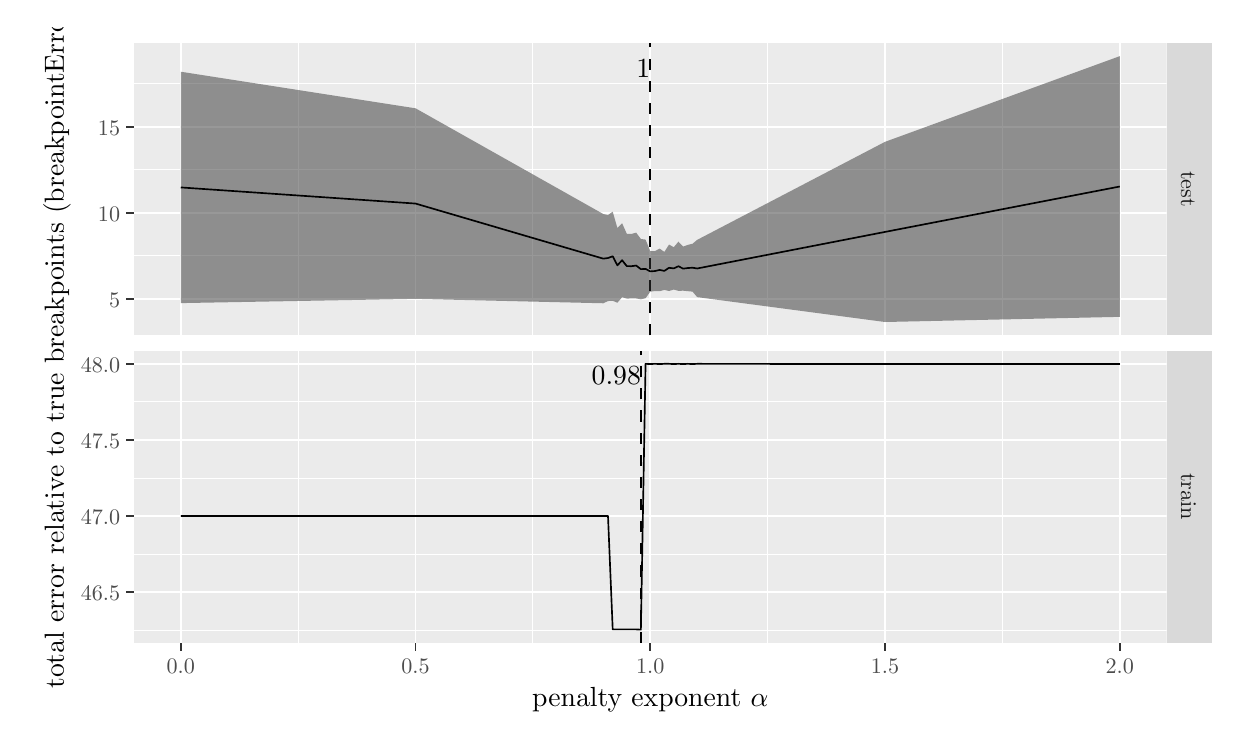
\begin{tikzpicture}[x=1pt,y=1pt]
\definecolor{fillColor}{RGB}{255,255,255}
\path[use as bounding box,fill=fillColor,fill opacity=0.00] (0,0) rectangle (433.62,252.94);
\begin{scope}
\path[clip] (  0.00,  0.00) rectangle (433.62,252.94);
\definecolor{drawColor}{RGB}{255,255,255}
\definecolor{fillColor}{RGB}{255,255,255}

\path[draw=drawColor,line width= 0.6pt,line join=round,line cap=round,fill=fillColor] (  0.00,  0.00) rectangle (433.62,252.94);
\end{scope}
\begin{scope}
\path[clip] ( 38.36,141.78) rectangle (411.58,247.45);
\definecolor{fillColor}{gray}{0.92}

\path[fill=fillColor] ( 38.36,141.78) rectangle (411.58,247.45);
\definecolor{drawColor}{RGB}{255,255,255}

\path[draw=drawColor,line width= 0.3pt,line join=round] ( 38.36,170.50) --
	(411.58,170.50);

\path[draw=drawColor,line width= 0.3pt,line join=round] ( 38.36,201.58) --
	(411.58,201.58);

\path[draw=drawColor,line width= 0.3pt,line join=round] ( 38.36,232.65) --
	(411.58,232.65);

\path[draw=drawColor,line width= 0.3pt,line join=round] ( 97.73,141.78) --
	( 97.73,247.45);

\path[draw=drawColor,line width= 0.3pt,line join=round] (182.56,141.78) --
	(182.56,247.45);

\path[draw=drawColor,line width= 0.3pt,line join=round] (267.38,141.78) --
	(267.38,247.45);

\path[draw=drawColor,line width= 0.3pt,line join=round] (352.21,141.78) --
	(352.21,247.45);

\path[draw=drawColor,line width= 0.6pt,line join=round] ( 38.36,154.96) --
	(411.58,154.96);

\path[draw=drawColor,line width= 0.6pt,line join=round] ( 38.36,186.04) --
	(411.58,186.04);

\path[draw=drawColor,line width= 0.6pt,line join=round] ( 38.36,217.12) --
	(411.58,217.12);

\path[draw=drawColor,line width= 0.6pt,line join=round] ( 55.32,141.78) --
	( 55.32,247.45);

\path[draw=drawColor,line width= 0.6pt,line join=round] (140.15,141.78) --
	(140.15,247.45);

\path[draw=drawColor,line width= 0.6pt,line join=round] (224.97,141.78) --
	(224.97,247.45);

\path[draw=drawColor,line width= 0.6pt,line join=round] (309.79,141.78) --
	(309.79,247.45);

\path[draw=drawColor,line width= 0.6pt,line join=round] (394.62,141.78) --
	(394.62,247.45);
\definecolor{drawColor}{RGB}{0,0,0}

\path[draw=drawColor,line width= 0.6pt,dash pattern=on 4pt off 4pt ,line join=round] (224.97,141.78) -- (224.97,247.45);

\node[text=drawColor,anchor=base east,inner sep=0pt, outer sep=0pt, scale=  1.00] at (224.97,235.07) {1};
\definecolor{fillColor}{RGB}{51,51,51}

\path[fill=fillColor,fill opacity=0.50] ( 55.32,237.02) --
	(140.15,223.80) --
	(208.01,185.59) --
	(209.70,185.25) --
	(211.40,186.44) --
	(213.09,180.55) --
	(214.79,182.28) --
	(216.49,178.47) --
	(218.18,178.40) --
	(219.88,178.87) --
	(221.58,176.57) --
	(223.27,176.36) --
	(224.97,172.21) --
	(226.67,172.22) --
	(228.36,173.10) --
	(230.06,171.91) --
	(231.76,174.57) --
	(233.45,173.60) --
	(235.15,175.61) --
	(236.85,173.83) --
	(238.54,174.44) --
	(240.24,174.86) --
	(241.94,176.27) --
	(309.79,211.68) --
	(394.62,242.64) --
	(394.62,148.44) --
	(309.79,146.58) --
	(241.94,155.57) --
	(240.24,157.55) --
	(238.54,157.72) --
	(236.85,157.89) --
	(235.15,157.84) --
	(233.45,158.30) --
	(231.76,157.78) --
	(230.06,158.18) --
	(228.36,157.71) --
	(226.67,157.78) --
	(224.97,157.54) --
	(223.27,155.17) --
	(221.58,154.79) --
	(219.88,155.09) --
	(218.18,155.09) --
	(216.49,155.06) --
	(214.79,155.52) --
	(213.09,153.54) --
	(211.40,154.25) --
	(209.70,154.15) --
	(208.01,153.35) --
	(140.15,154.95) --
	( 55.32,153.41) --
	cycle;

\path[] ( 55.32,237.02) --
	(140.15,223.80) --
	(208.01,185.59) --
	(209.70,185.25) --
	(211.40,186.44) --
	(213.09,180.55) --
	(214.79,182.28) --
	(216.49,178.47) --
	(218.18,178.40) --
	(219.88,178.87) --
	(221.58,176.57) --
	(223.27,176.36) --
	(224.97,172.21) --
	(226.67,172.22) --
	(228.36,173.10) --
	(230.06,171.91) --
	(231.76,174.57) --
	(233.45,173.60) --
	(235.15,175.61) --
	(236.85,173.83) --
	(238.54,174.44) --
	(240.24,174.86) --
	(241.94,176.27) --
	(309.79,211.68) --
	(394.62,242.64);

\path[] (394.62,148.44) --
	(309.79,146.58) --
	(241.94,155.57) --
	(240.24,157.55) --
	(238.54,157.72) --
	(236.85,157.89) --
	(235.15,157.84) --
	(233.45,158.30) --
	(231.76,157.78) --
	(230.06,158.18) --
	(228.36,157.71) --
	(226.67,157.78) --
	(224.97,157.54) --
	(223.27,155.17) --
	(221.58,154.79) --
	(219.88,155.09) --
	(218.18,155.09) --
	(216.49,155.06) --
	(214.79,155.52) --
	(213.09,153.54) --
	(211.40,154.25) --
	(209.70,154.15) --
	(208.01,153.35) --
	(140.15,154.95) --
	( 55.32,153.41);

\path[draw=drawColor,line width= 0.6pt,line join=round] ( 55.32,195.21) --
	(140.15,189.38) --
	(208.01,169.47) --
	(209.70,169.70) --
	(211.40,170.34) --
	(213.09,167.05) --
	(214.79,168.90) --
	(216.49,166.77) --
	(218.18,166.75) --
	(219.88,166.98) --
	(221.58,165.68) --
	(223.27,165.76) --
	(224.97,164.87) --
	(226.67,165.00) --
	(228.36,165.40) --
	(230.06,165.05) --
	(231.76,166.17) --
	(233.45,165.95) --
	(235.15,166.73) --
	(236.85,165.86) --
	(238.54,166.08) --
	(240.24,166.20) --
	(241.94,165.92) --
	(309.79,179.13) --
	(394.62,195.54);
\end{scope}
\begin{scope}
\path[clip] ( 38.36, 30.61) rectangle (411.58,136.28);
\definecolor{fillColor}{gray}{0.92}

\path[fill=fillColor] ( 38.36, 30.61) rectangle (411.58,136.28);
\definecolor{drawColor}{RGB}{255,255,255}

\path[draw=drawColor,line width= 0.3pt,line join=round] ( 38.36, 35.19) --
	(411.58, 35.19);

\path[draw=drawColor,line width= 0.3pt,line join=round] ( 38.36, 62.70) --
	(411.58, 62.70);

\path[draw=drawColor,line width= 0.3pt,line join=round] ( 38.36, 90.21) --
	(411.58, 90.21);

\path[draw=drawColor,line width= 0.3pt,line join=round] ( 38.36,117.72) --
	(411.58,117.72);

\path[draw=drawColor,line width= 0.3pt,line join=round] ( 97.73, 30.61) --
	( 97.73,136.28);

\path[draw=drawColor,line width= 0.3pt,line join=round] (182.56, 30.61) --
	(182.56,136.28);

\path[draw=drawColor,line width= 0.3pt,line join=round] (267.38, 30.61) --
	(267.38,136.28);

\path[draw=drawColor,line width= 0.3pt,line join=round] (352.21, 30.61) --
	(352.21,136.28);

\path[draw=drawColor,line width= 0.6pt,line join=round] ( 38.36, 48.94) --
	(411.58, 48.94);

\path[draw=drawColor,line width= 0.6pt,line join=round] ( 38.36, 76.45) --
	(411.58, 76.45);

\path[draw=drawColor,line width= 0.6pt,line join=round] ( 38.36,103.96) --
	(411.58,103.96);

\path[draw=drawColor,line width= 0.6pt,line join=round] ( 38.36,131.47) --
	(411.58,131.47);

\path[draw=drawColor,line width= 0.6pt,line join=round] ( 55.32, 30.61) --
	( 55.32,136.28);

\path[draw=drawColor,line width= 0.6pt,line join=round] (140.15, 30.61) --
	(140.15,136.28);

\path[draw=drawColor,line width= 0.6pt,line join=round] (224.97, 30.61) --
	(224.97,136.28);

\path[draw=drawColor,line width= 0.6pt,line join=round] (309.79, 30.61) --
	(309.79,136.28);

\path[draw=drawColor,line width= 0.6pt,line join=round] (394.62, 30.61) --
	(394.62,136.28);
\definecolor{drawColor}{RGB}{0,0,0}

\path[draw=drawColor,line width= 0.6pt,dash pattern=on 4pt off 4pt ,line join=round] (221.58, 30.61) -- (221.58,136.28);

\node[text=drawColor,anchor=base east,inner sep=0pt, outer sep=0pt, scale=  1.00] at (221.58,123.90) {0.98};

\path[draw=drawColor,line width= 0.6pt,line join=round] ( 55.32, 76.46) --
	(140.15, 76.46) --
	(208.01, 76.46) --
	(209.70, 76.46) --
	(211.40, 35.50) --
	(213.09, 35.50) --
	(214.79, 35.50) --
	(216.49, 35.50) --
	(218.18, 35.50) --
	(219.88, 35.50) --
	(221.58, 35.41) --
	(223.27,131.47) --
	(224.97,131.38) --
	(226.67,131.47) --
	(228.36,131.38) --
	(230.06,131.47) --
	(231.76,131.47) --
	(233.45,131.38) --
	(235.15,131.47) --
	(236.85,131.38) --
	(238.54,131.47) --
	(240.24,131.38) --
	(241.94,131.47) --
	(309.79,131.38) --
	(394.62,131.38);
\end{scope}
\begin{scope}
\path[clip] (411.58,141.78) rectangle (428.12,247.45);
\definecolor{fillColor}{gray}{0.85}

\path[fill=fillColor] (411.58,141.78) rectangle (428.12,247.45);
\definecolor{drawColor}{gray}{0.10}

\node[text=drawColor,rotate=-90.00,anchor=base,inner sep=0pt, outer sep=0pt, scale=  0.80] at (416.84,194.61) {test};
\end{scope}
\begin{scope}
\path[clip] (411.58, 30.61) rectangle (428.12,136.28);
\definecolor{fillColor}{gray}{0.85}

\path[fill=fillColor] (411.58, 30.61) rectangle (428.12,136.28);
\definecolor{drawColor}{gray}{0.10}

\node[text=drawColor,rotate=-90.00,anchor=base,inner sep=0pt, outer sep=0pt, scale=  0.80] at (416.84, 83.44) {train};
\end{scope}
\begin{scope}
\path[clip] (  0.00,  0.00) rectangle (433.62,252.94);
\definecolor{drawColor}{gray}{0.20}

\path[draw=drawColor,line width= 0.6pt,line join=round] ( 55.32, 27.86) --
	( 55.32, 30.61);

\path[draw=drawColor,line width= 0.6pt,line join=round] (140.15, 27.86) --
	(140.15, 30.61);

\path[draw=drawColor,line width= 0.6pt,line join=round] (224.97, 27.86) --
	(224.97, 30.61);

\path[draw=drawColor,line width= 0.6pt,line join=round] (309.79, 27.86) --
	(309.79, 30.61);

\path[draw=drawColor,line width= 0.6pt,line join=round] (394.62, 27.86) --
	(394.62, 30.61);
\end{scope}
\begin{scope}
\path[clip] (  0.00,  0.00) rectangle (433.62,252.94);
\definecolor{drawColor}{gray}{0.30}

\node[text=drawColor,anchor=base,inner sep=0pt, outer sep=0pt, scale=  0.80] at ( 55.32, 19.62) {0.0};

\node[text=drawColor,anchor=base,inner sep=0pt, outer sep=0pt, scale=  0.80] at (140.15, 19.62) {0.5};

\node[text=drawColor,anchor=base,inner sep=0pt, outer sep=0pt, scale=  0.80] at (224.97, 19.62) {1.0};

\node[text=drawColor,anchor=base,inner sep=0pt, outer sep=0pt, scale=  0.80] at (309.79, 19.62) {1.5};

\node[text=drawColor,anchor=base,inner sep=0pt, outer sep=0pt, scale=  0.80] at (394.62, 19.62) {2.0};
\end{scope}
\begin{scope}
\path[clip] (  0.00,  0.00) rectangle (433.62,252.94);
\definecolor{drawColor}{gray}{0.30}

\node[text=drawColor,anchor=base east,inner sep=0pt, outer sep=0pt, scale=  0.80] at ( 33.41,151.94) {5};

\node[text=drawColor,anchor=base east,inner sep=0pt, outer sep=0pt, scale=  0.80] at ( 33.41,183.02) {10};

\node[text=drawColor,anchor=base east,inner sep=0pt, outer sep=0pt, scale=  0.80] at ( 33.41,214.10) {15};
\end{scope}
\begin{scope}
\path[clip] (  0.00,  0.00) rectangle (433.62,252.94);
\definecolor{drawColor}{gray}{0.20}

\path[draw=drawColor,line width= 0.6pt,line join=round] ( 35.61,154.96) --
	( 38.36,154.96);

\path[draw=drawColor,line width= 0.6pt,line join=round] ( 35.61,186.04) --
	( 38.36,186.04);

\path[draw=drawColor,line width= 0.6pt,line join=round] ( 35.61,217.12) --
	( 38.36,217.12);
\end{scope}
\begin{scope}
\path[clip] (  0.00,  0.00) rectangle (433.62,252.94);
\definecolor{drawColor}{gray}{0.30}

\node[text=drawColor,anchor=base east,inner sep=0pt, outer sep=0pt, scale=  0.80] at ( 33.41, 45.93) {46.5};

\node[text=drawColor,anchor=base east,inner sep=0pt, outer sep=0pt, scale=  0.80] at ( 33.41, 73.44) {47.0};

\node[text=drawColor,anchor=base east,inner sep=0pt, outer sep=0pt, scale=  0.80] at ( 33.41,100.95) {47.5};

\node[text=drawColor,anchor=base east,inner sep=0pt, outer sep=0pt, scale=  0.80] at ( 33.41,128.46) {48.0};
\end{scope}
\begin{scope}
\path[clip] (  0.00,  0.00) rectangle (433.62,252.94);
\definecolor{drawColor}{gray}{0.20}

\path[draw=drawColor,line width= 0.6pt,line join=round] ( 35.61, 48.94) --
	( 38.36, 48.94);

\path[draw=drawColor,line width= 0.6pt,line join=round] ( 35.61, 76.45) --
	( 38.36, 76.45);

\path[draw=drawColor,line width= 0.6pt,line join=round] ( 35.61,103.96) --
	( 38.36,103.96);

\path[draw=drawColor,line width= 0.6pt,line join=round] ( 35.61,131.47) --
	( 38.36,131.47);
\end{scope}
\begin{scope}
\path[clip] (  0.00,  0.00) rectangle (433.62,252.94);
\definecolor{drawColor}{RGB}{0,0,0}

\node[text=drawColor,anchor=base,inner sep=0pt, outer sep=0pt, scale=  1.00] at (224.97,  7.63) {penalty exponent $\alpha$};
\end{scope}
\begin{scope}
\path[clip] (  0.00,  0.00) rectangle (433.62,252.94);
\definecolor{drawColor}{RGB}{0,0,0}

\node[text=drawColor,rotate= 90.00,anchor=base,inner sep=0pt, outer sep=0pt, scale=  1.00] at ( 13.04,139.03) {total error relative to true breakpoints (breakpointError)};
\end{scope}
\end{tikzpicture}
